The experimental set-up consists of the following components: 
\begin{itemize}
\item laser.
\item focusing lens.
\item beam splitter.
\item pendulum.
\item two photodiodes.
\item circuit, ADC, PC.
\end{itemize}
All these items are arranged according to the schematic in fig. \ref{fig:expsetup} and fig. \ref{fig:expsetupLive} shows the real system set-up.
\begin{figure}[htbp]
	\centering
	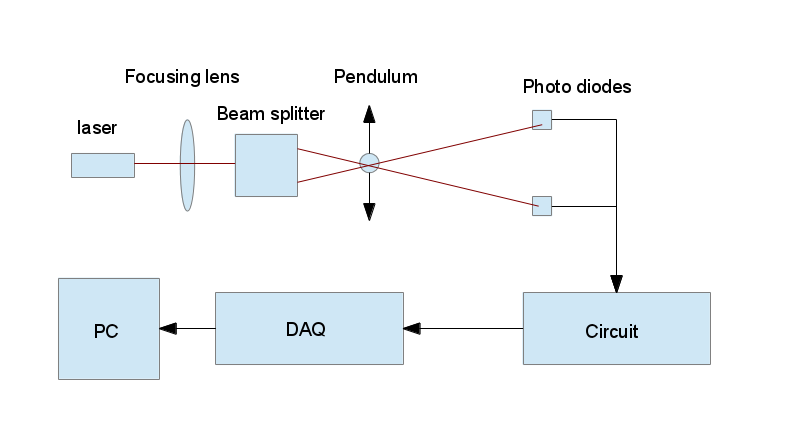
\includegraphics[width=0.8\textwidth]{img/expsetup}
	\caption{Schematic diagram of the experimental set-up. The laser is focused onto the pendulum by the focusing lens. Between focusing lens and the pendulum there is a beam splitter that splits the beam in to two beams that at the pendulum position are very narrowly separated. The photo diodes converts the beam into an electrical signal that goes in to the PC through an ADC.}
	\label{fig:expsetup}
\end{figure}
\begin{figure}[htbp]
	\centering
	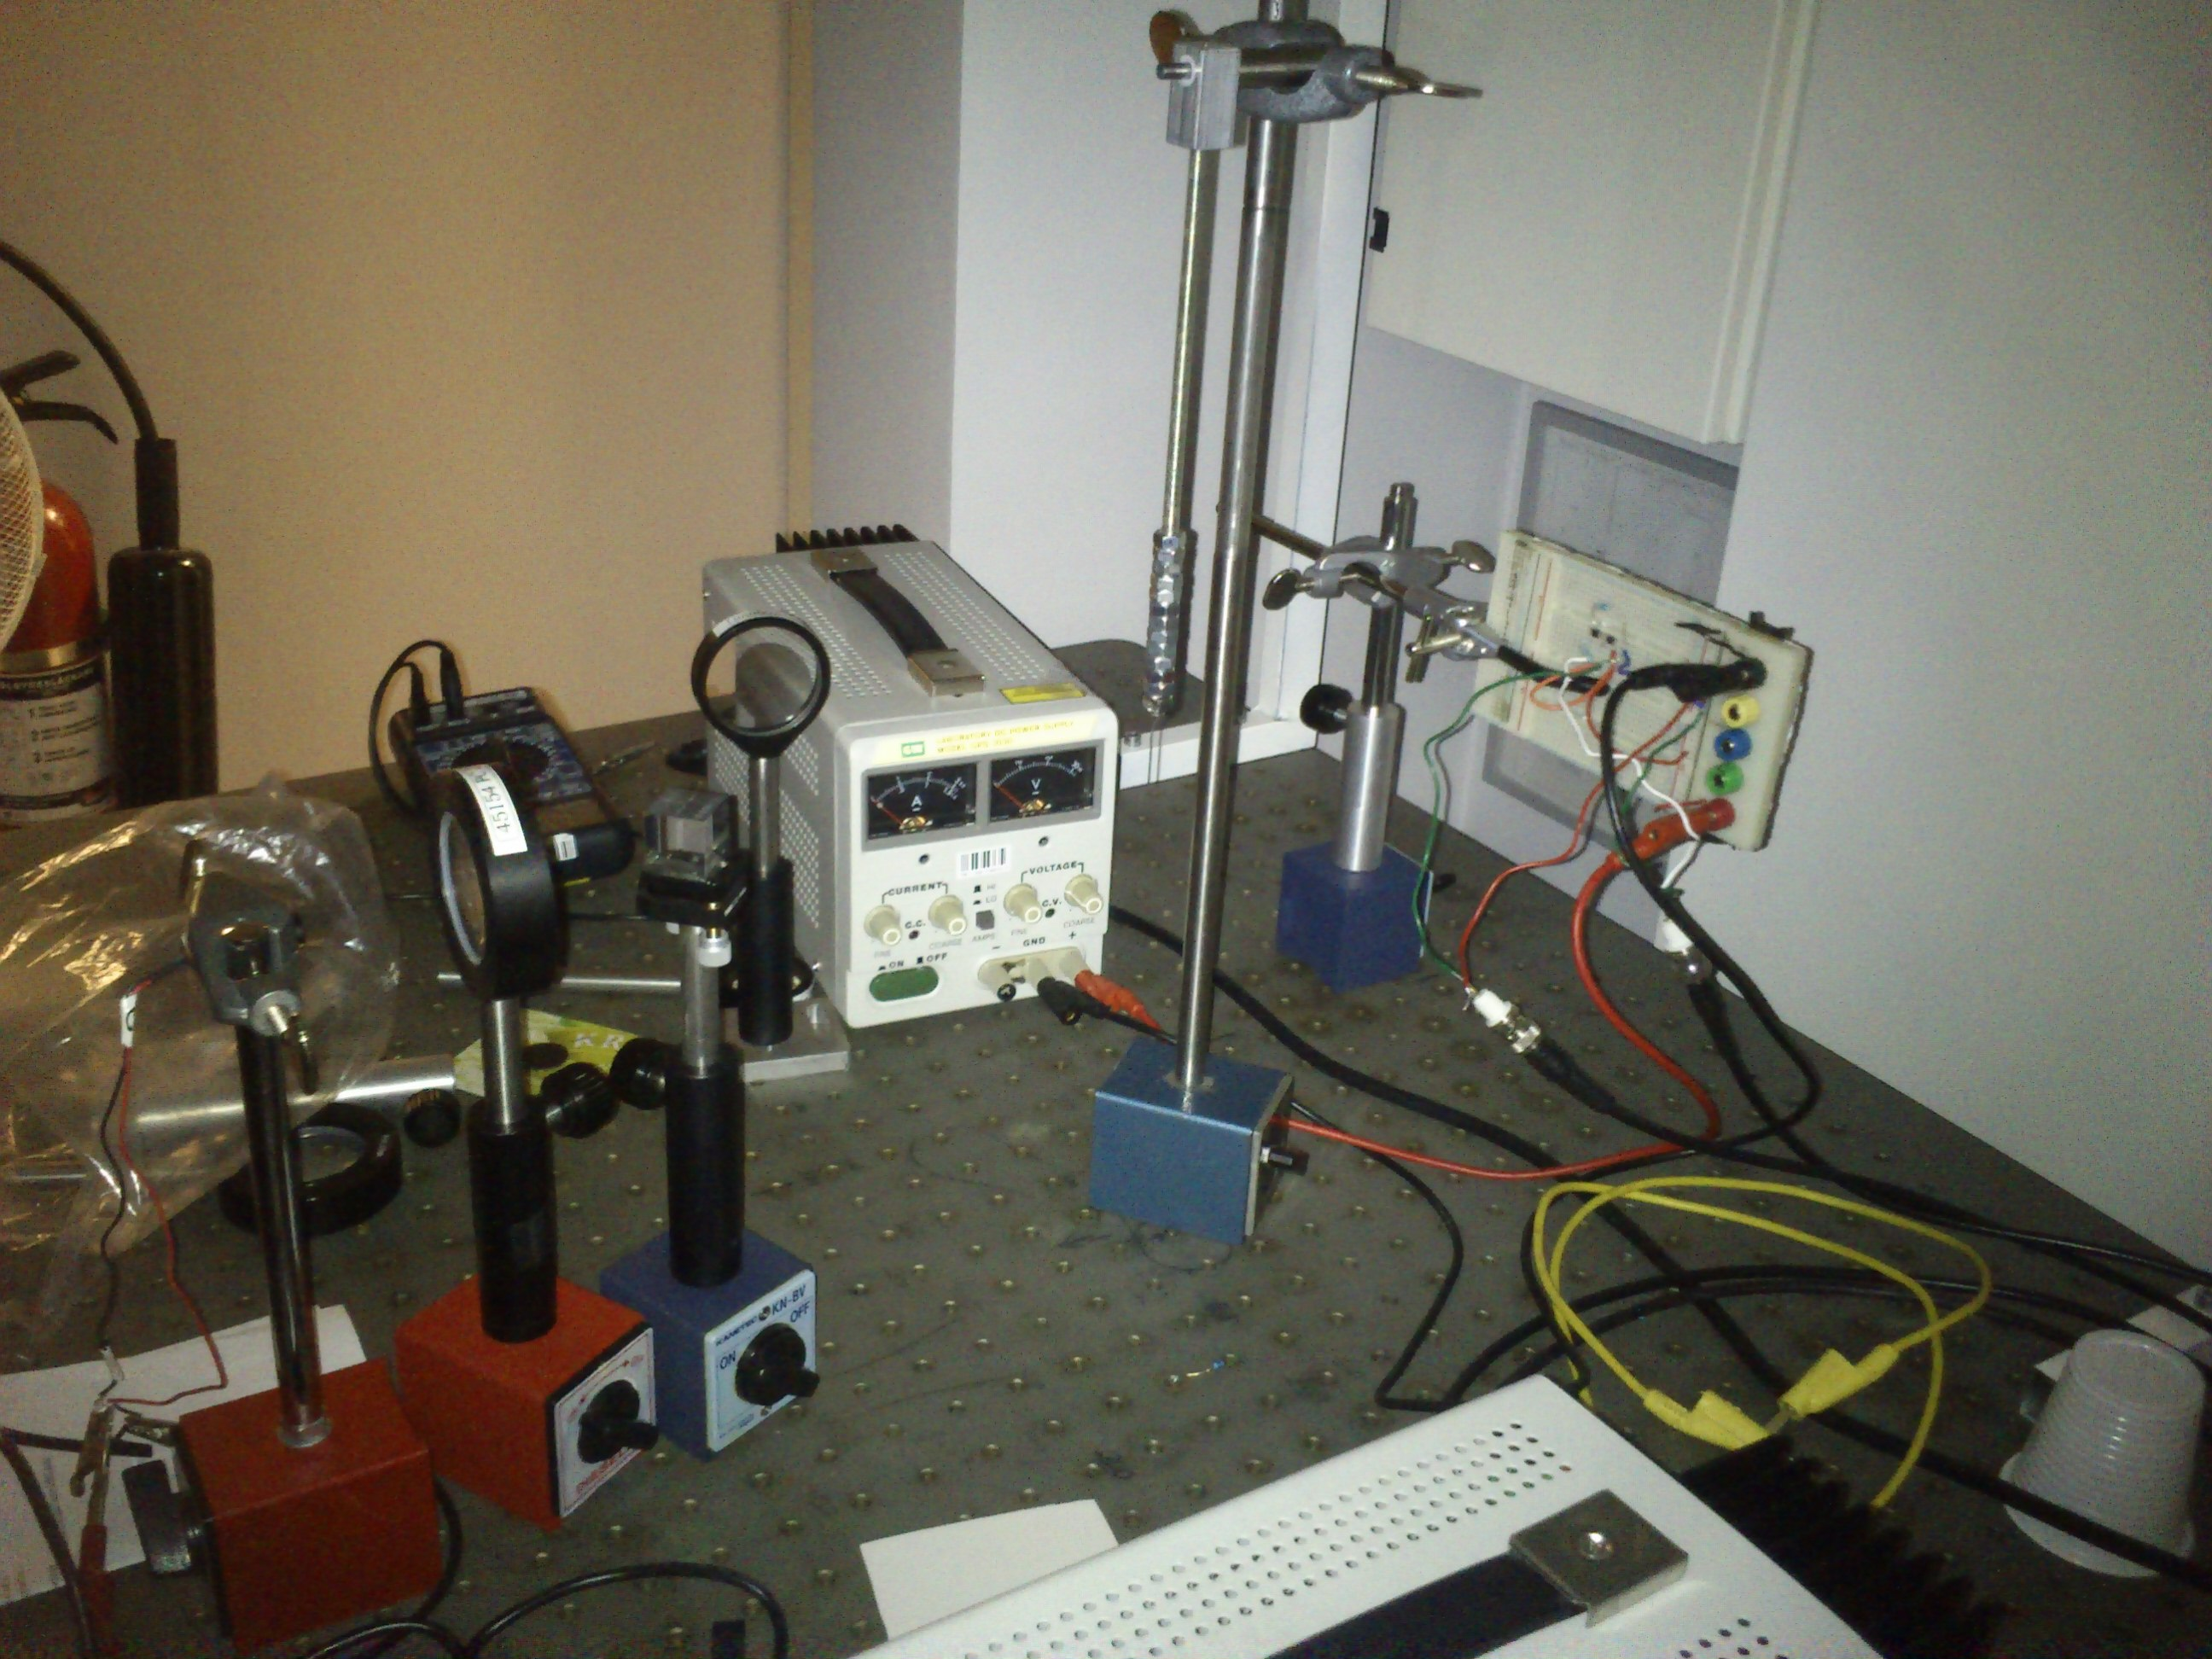
\includegraphics[width=0.8\textwidth]{img/expsetupLive}
	\caption{Real experimental setup. 1. Laser, 2. focusing lens, 3. beam splitter, 4. pendulum,
	5. photo diodes with circuit.} %TODO Add more info, number the components.
	\label{fig:expsetupLive}
\end{figure}
The two laser beams near the pendulum are covered by the pendulum at the different times meaning that there will be valleys in the output signal from the photo diodes at different times.
The velocity of the pendulum will be inversely proportional to the time difference of these two valleys measured by the photo diodes.

The two laser beams are directed at the point where the pendulum has its lowest potential energy or highest kinetic energy; and to get a good value for this velocity the two beams are at this point only separated by a distance of order of a millimetre in length.
Every time the pendulum swings by this point its total energy---which is the same as its kinetic energy---can be calculated and it will decay over time because of energy loss due to air drag and friction.

Since the separation of the two beams is very small we need a high sampling frequency to measure the velocity accurately; we used a sampling frequency of $100\;\rm{kHz}$ which means we can measure velocities in the order of 
%TODO fix this is to much
\mbox{$\approx 1\;\rm{mm} \cdot 100\;\rm{kHz} = 100 \rm{m/s}$}.
But since there is always some noise in the system the velocities which you can distinguish between is lower than this.

To see how the decay in energy of the pendulum depends on the friction, more mass can be added to the pendulum nearly without affecting the air drag, compare fig. \ref{fig:pendulumNormal} and fig. \ref{fig:pendulumHeavy}.
Similarly to examine the energy loss from air drag we changed the geometry of the pendulum, compare
fig. \ref{fig:pendulumNormal} and fig. \ref{fig:pendulumDraggy}.
%\begin{figure}[htbp]
%\begin{subfigure}
%	\centering
%	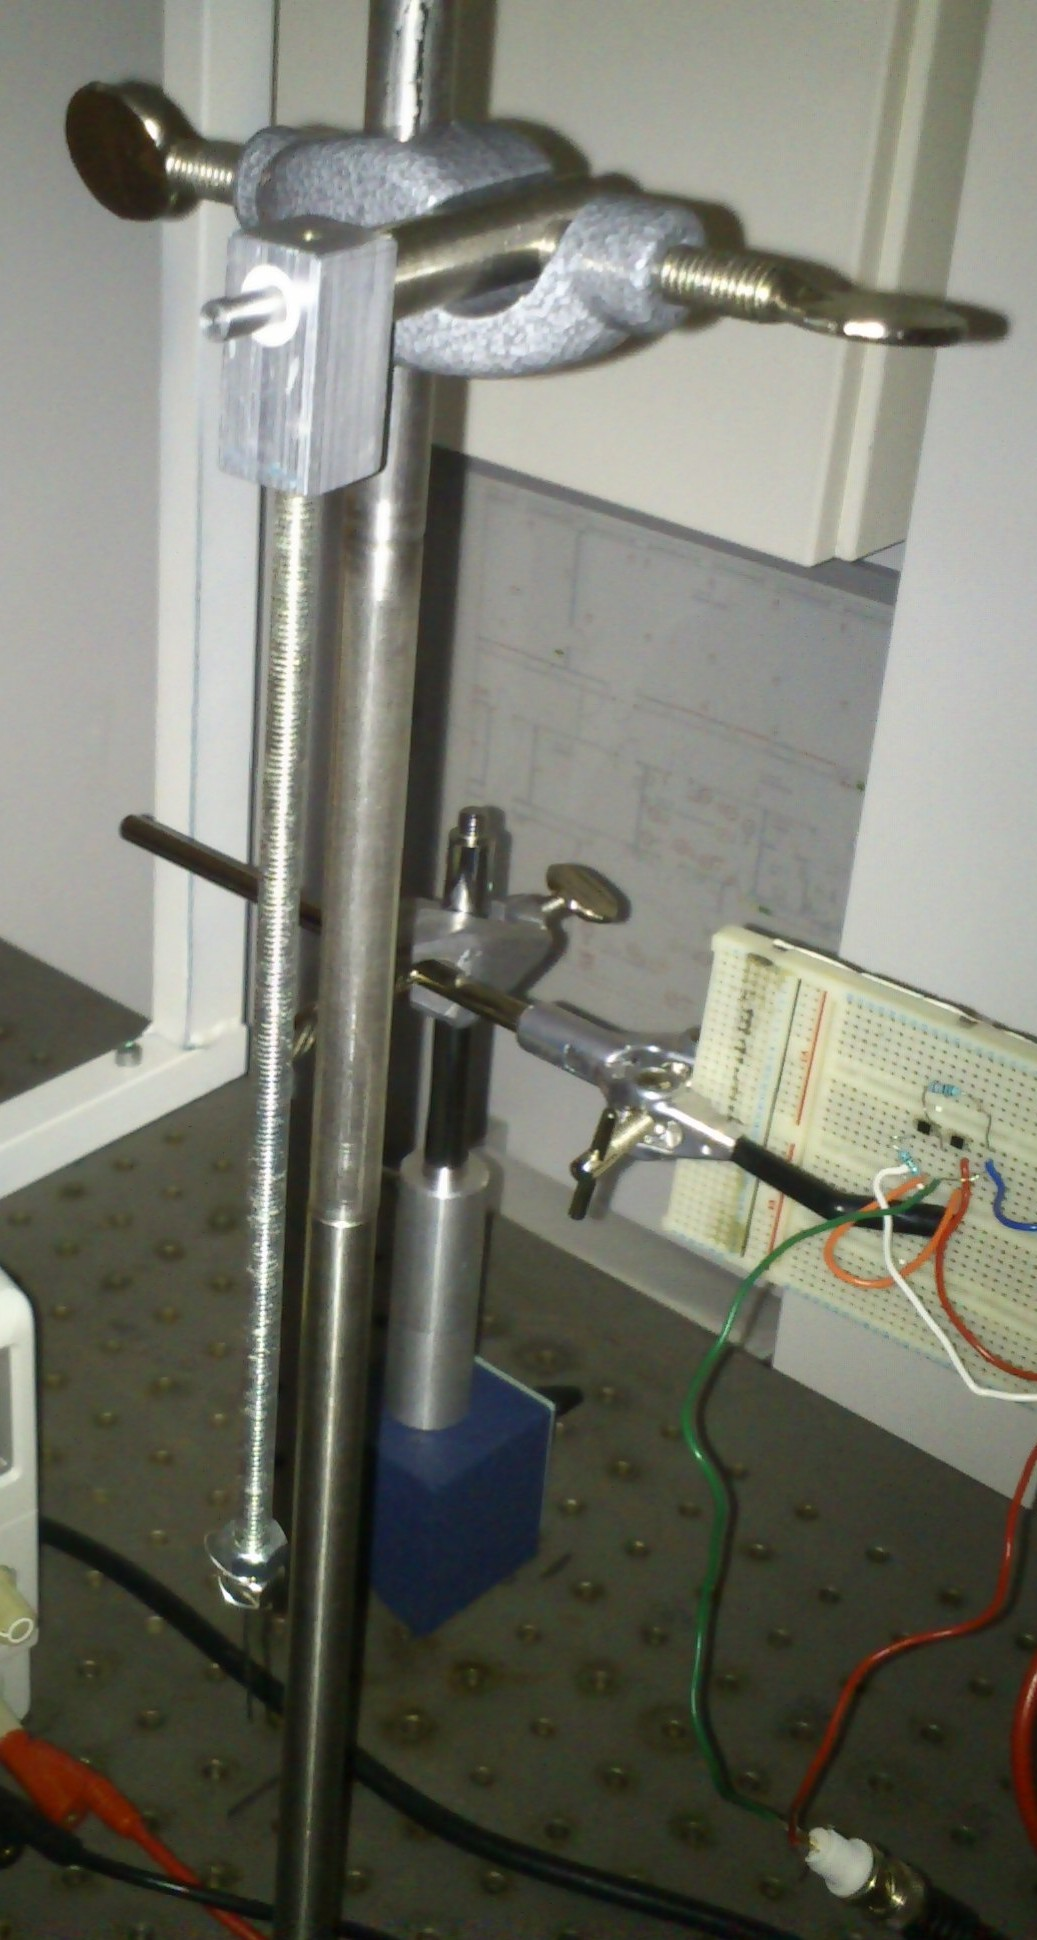
\includegraphics[width=0.50\textwidth]{img/pendulumNormal}
%	\caption{Normal weight and geometry of the  pendulum.}
%	\label{fig:pendulumNormal}
%\end{subfigure}
%\begin{subfigure}
%	\centering
%	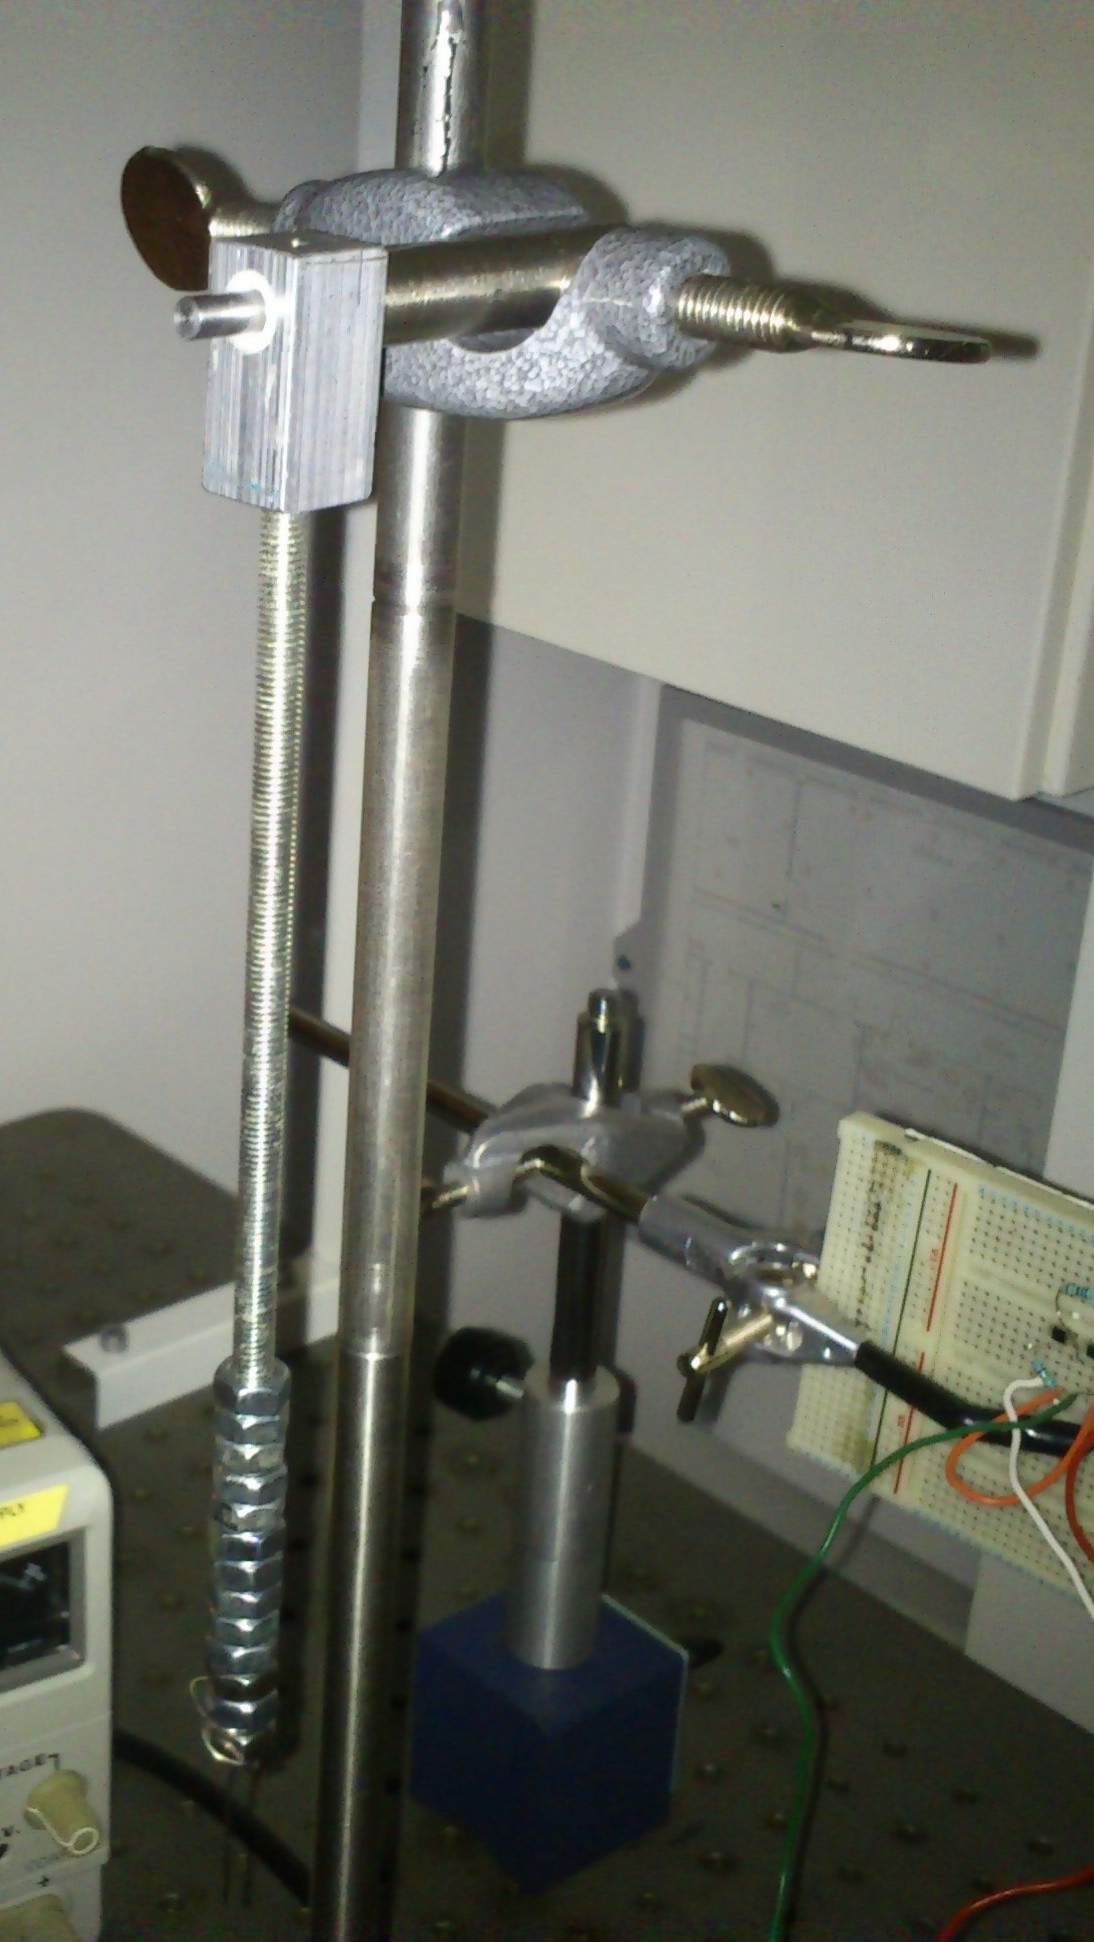
\includegraphics[width=0.50\textwidth]{img/pendulumHeavy}
%	\caption{Pendulum with added mass in the form of screw nuts.}
%	\label{fig:pendulumHeavy}
%\end{subfigure}
%\begin{subfigure}
%	\centering
%	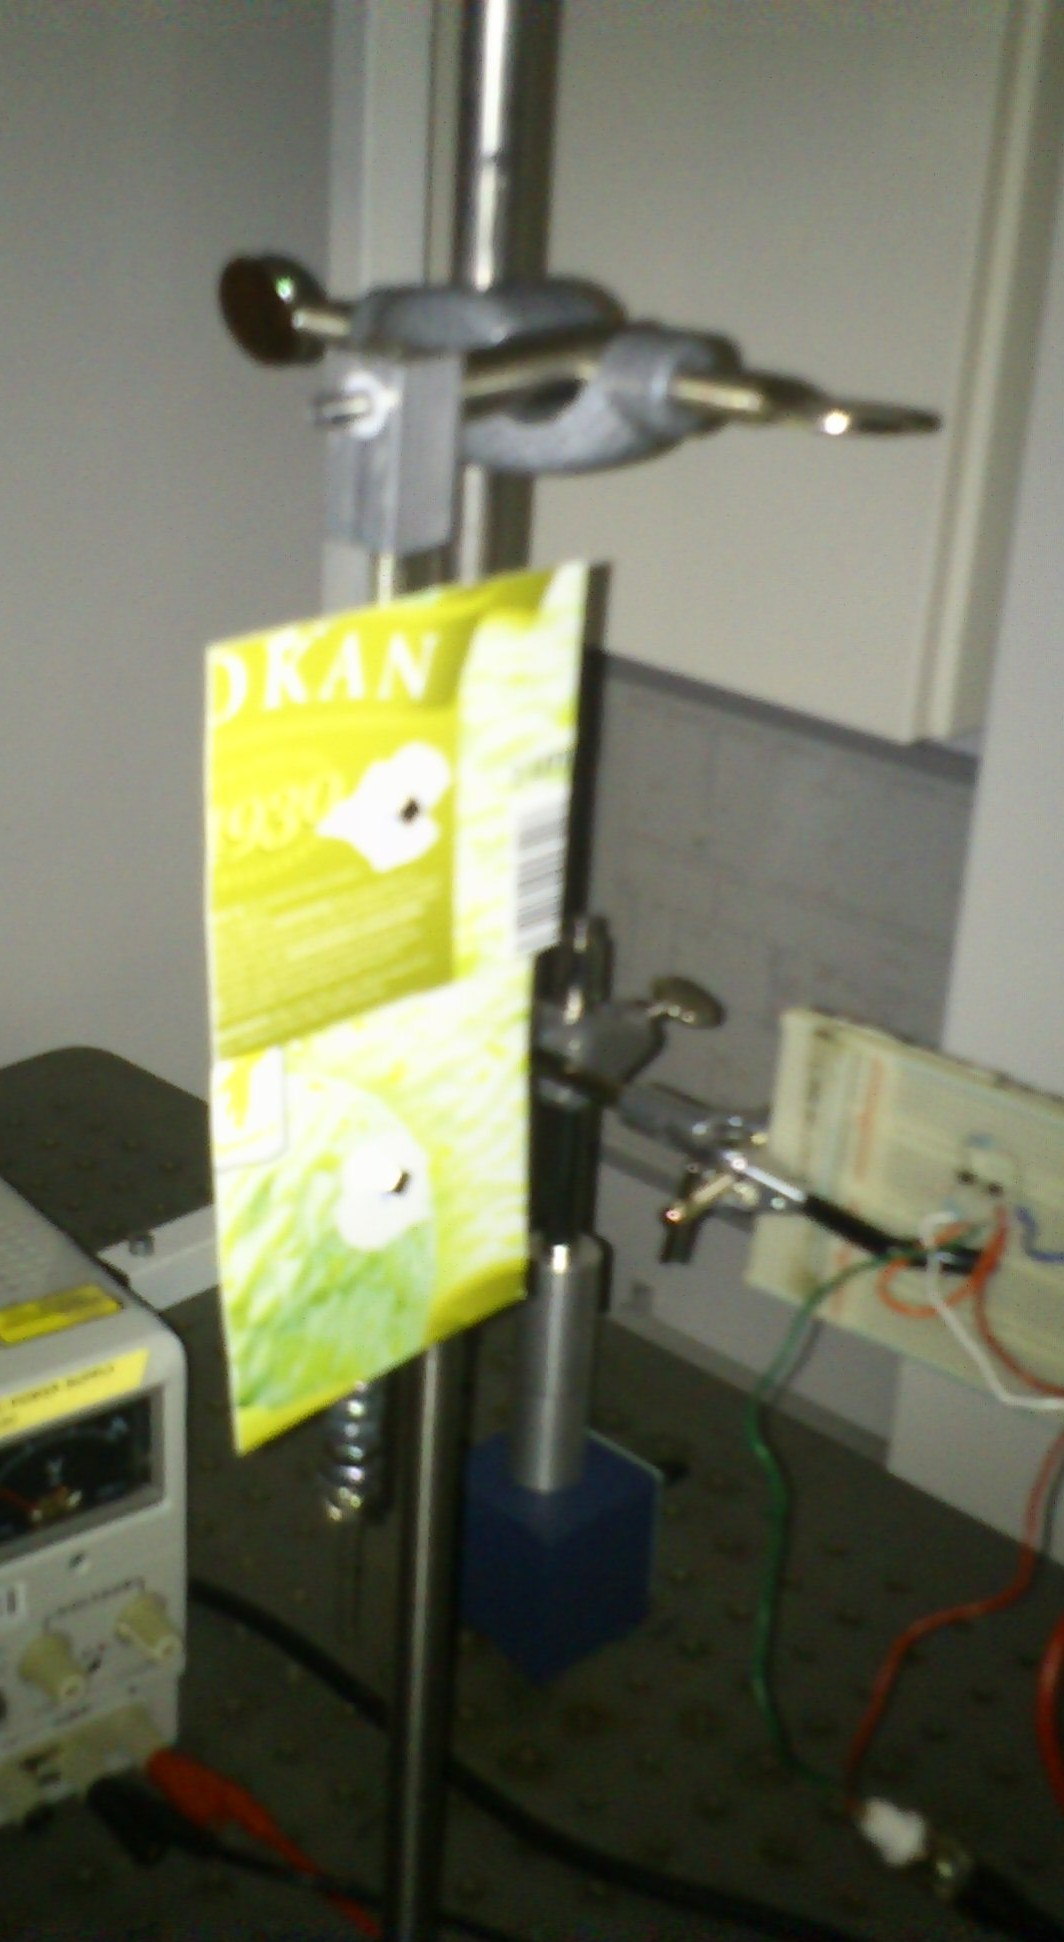
\includegraphics[width=0.50\textwidth]{img/pendulumDraggy}
%	\caption{Pendulum with increased air drag due to changed geometry.}
%	\label{fig:pendulumDraggy}
%\end{subfigure}
%\end{figure}



\begin{figure}[htbp]
\centering
\begin{subfigure}{.3\textwidth}
	\centering
	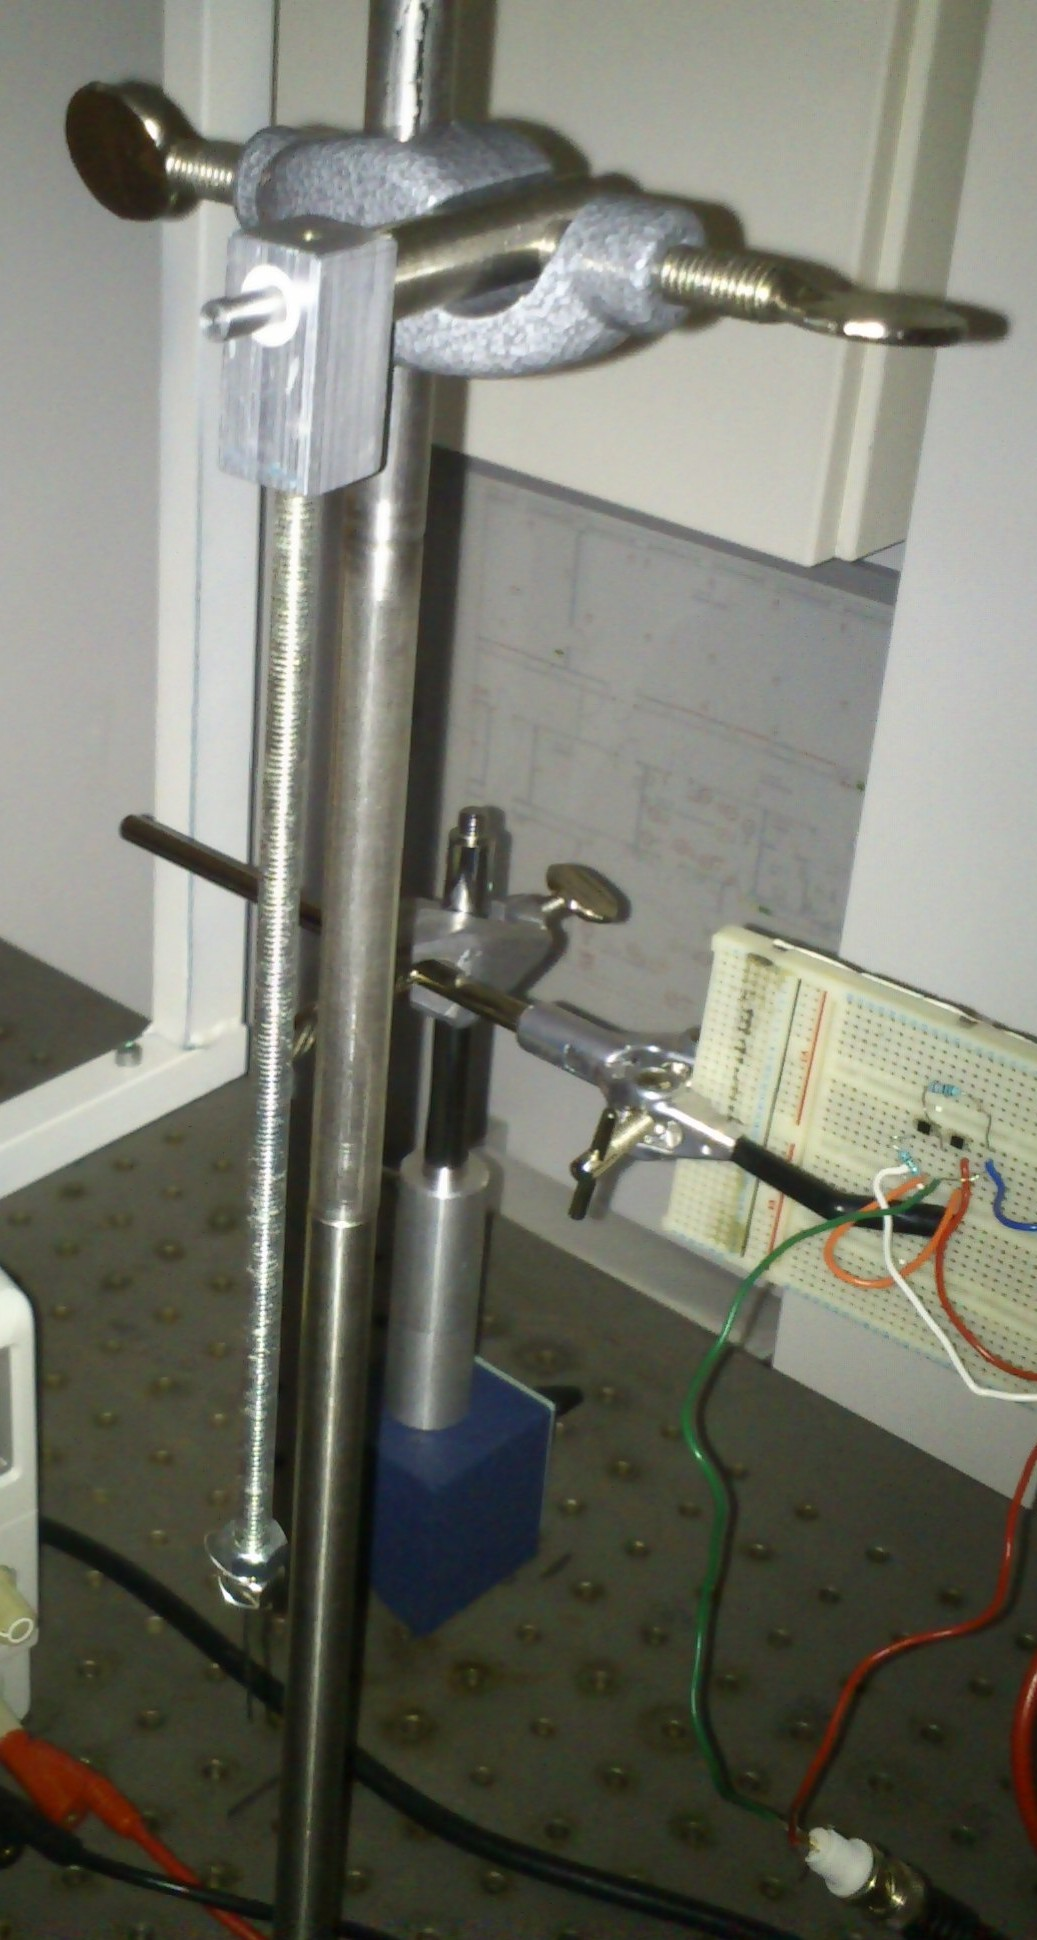
\includegraphics[width=\textwidth]{img/pendulumNormal}
	\caption{}
	\label{fig:pendulumNormal}
\end{subfigure}
\begin{subfigure}{.3\textwidth}
	\centering
	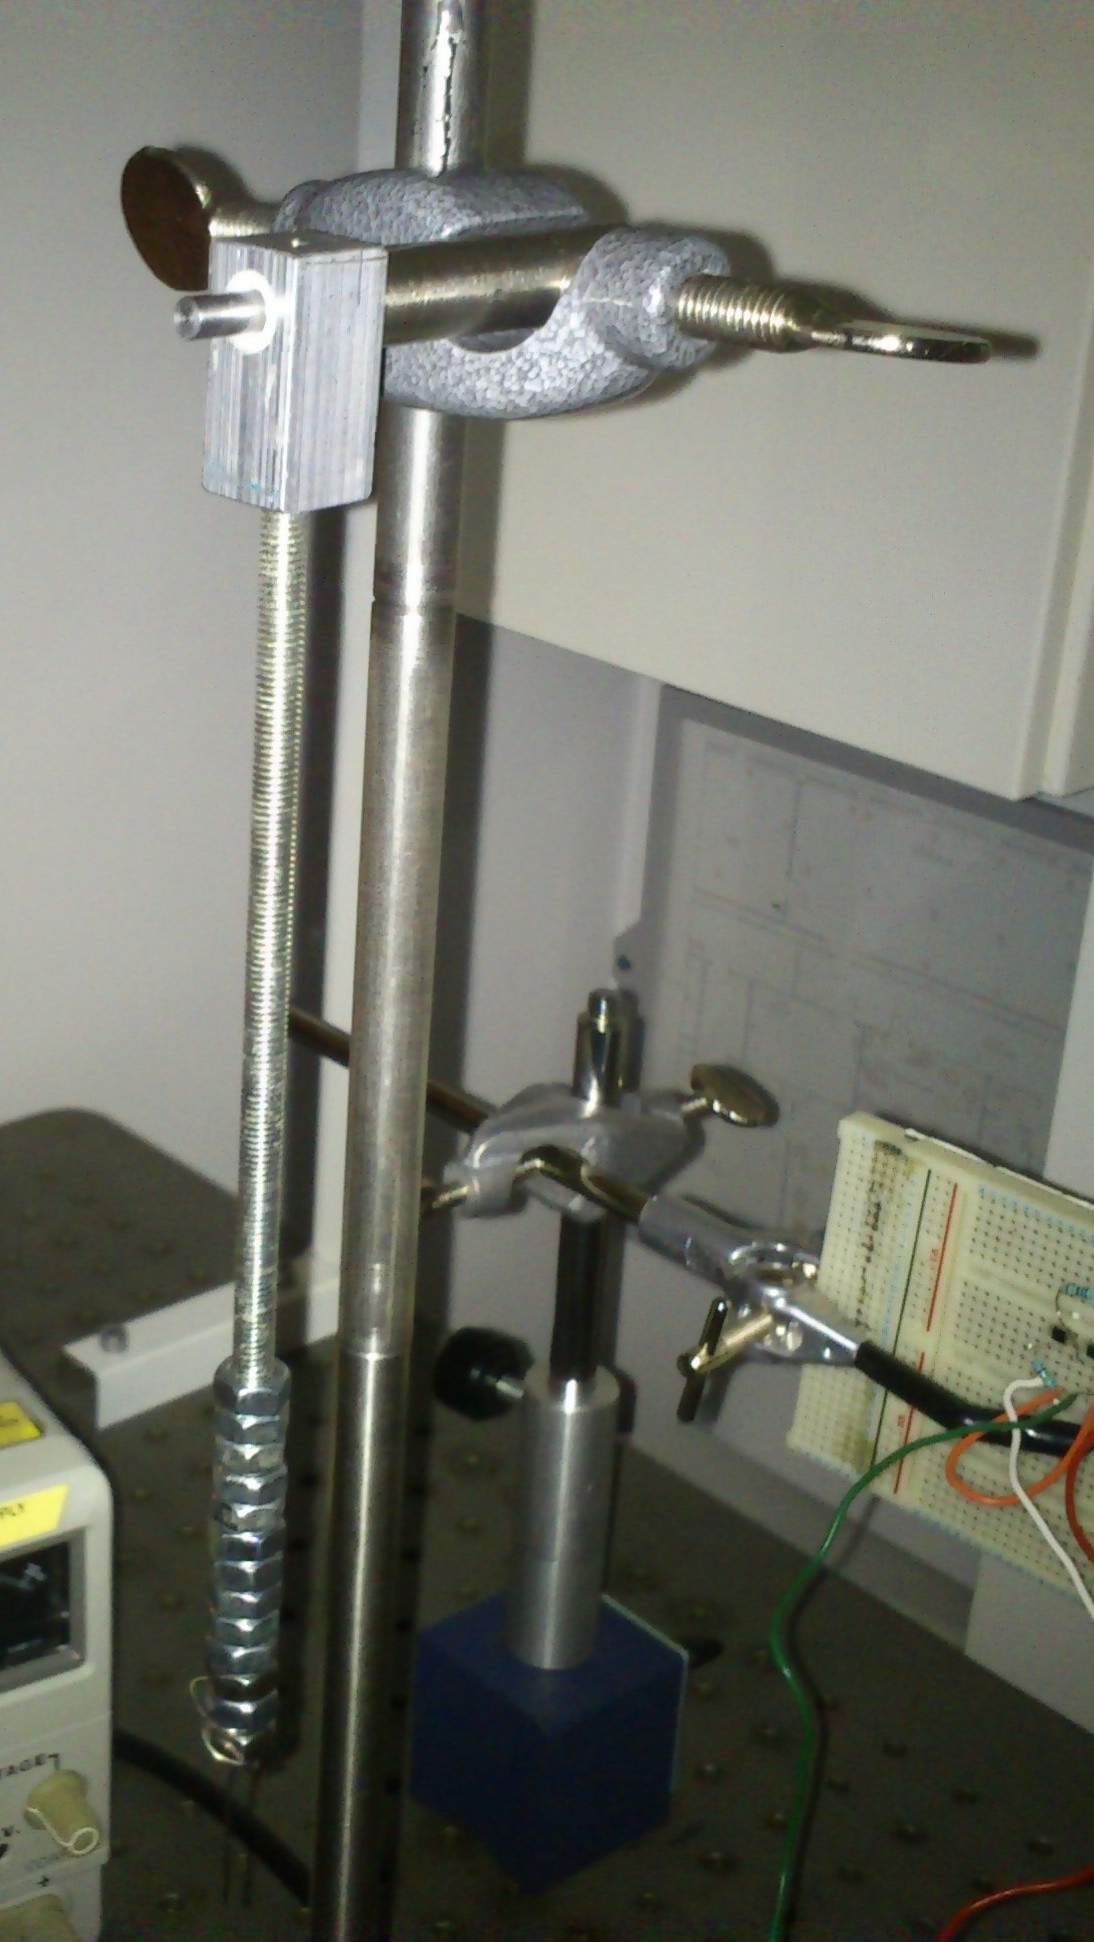
\includegraphics[width=\textwidth]{img/pendulumHeavy}
	\caption{}
	\label{fig:pendulumHeavy}
\end{subfigure}
\begin{subfigure}{.3\textwidth}
	\centering
	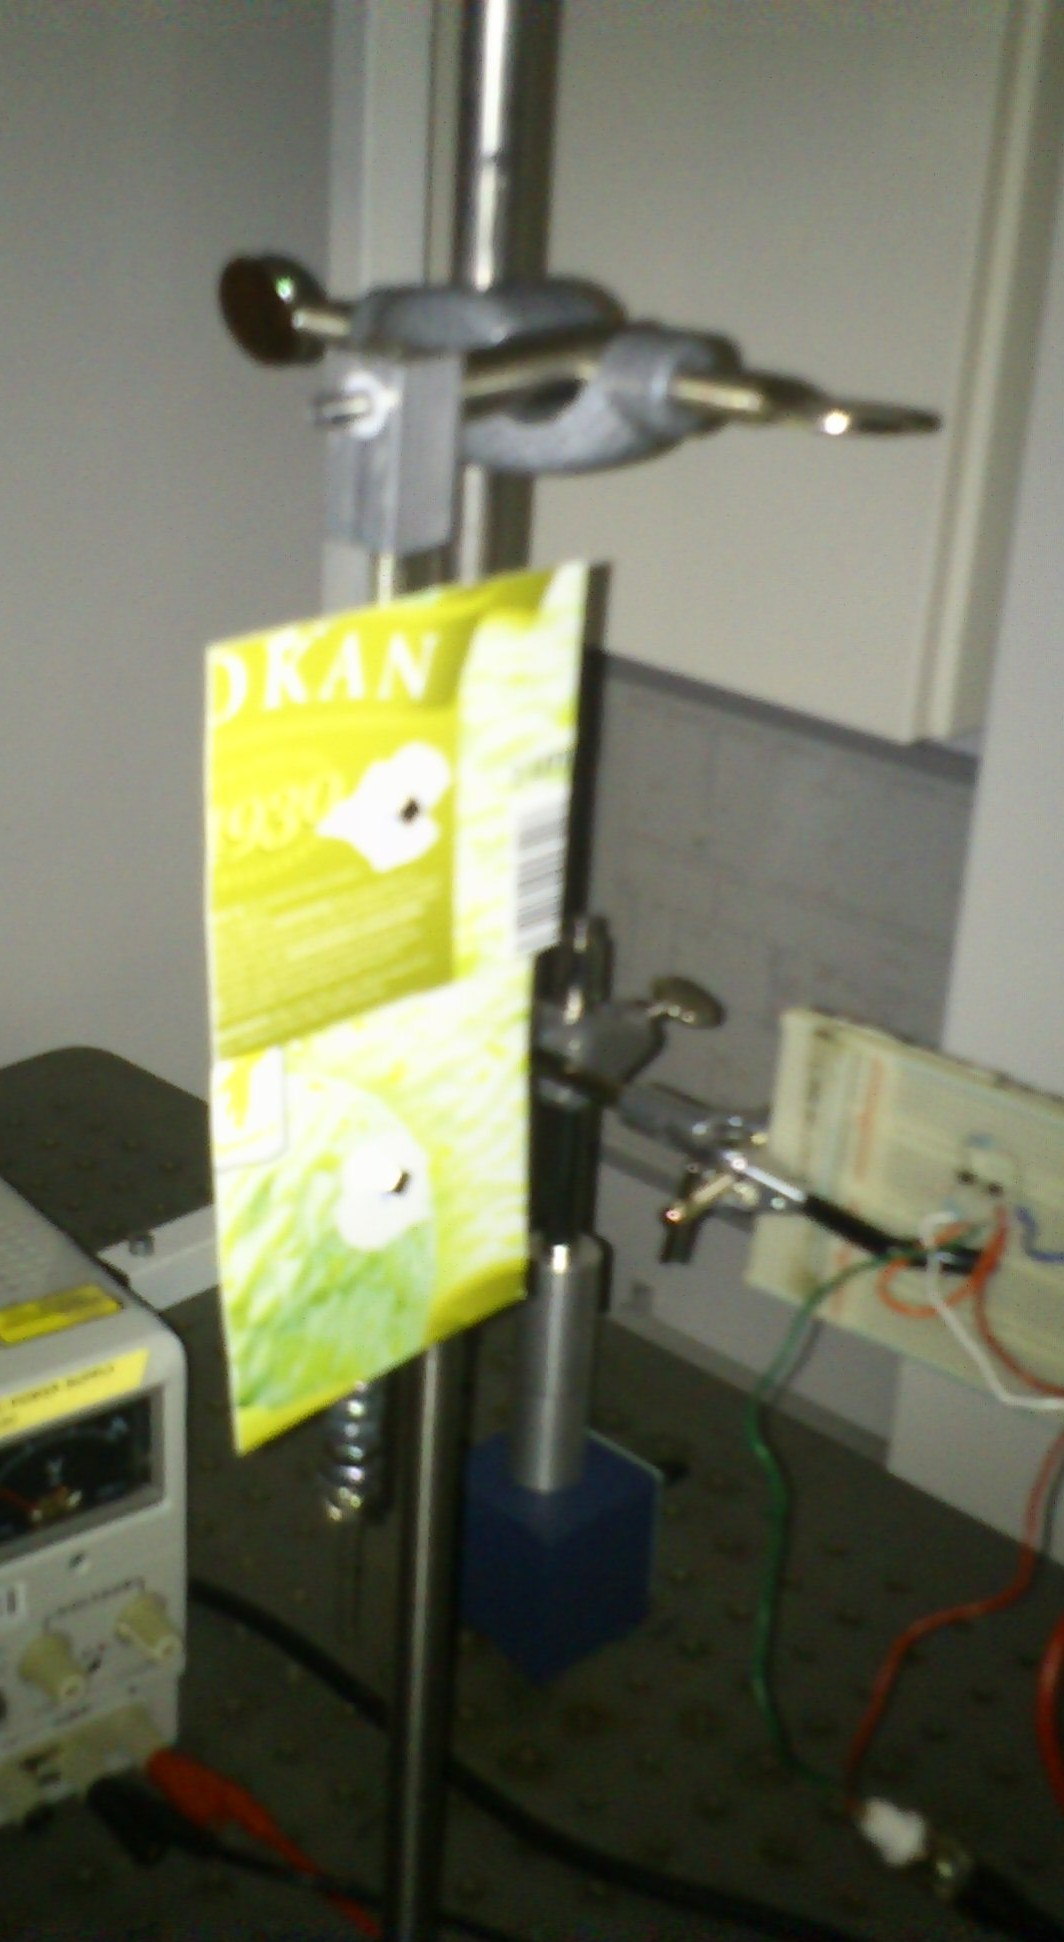
\includegraphics[width=\textwidth]{img/pendulumDraggy}
	\caption{}
	\label{fig:pendulumDraggy}
\end{subfigure}
\caption{(a) Normal weight and geometry of the  pendulum. (b) Pendulum with added mass in the form of screw nuts. (c) Pendulum with increased air drag due to changed geometry.}
\end{figure}